\documentclass[aspectratio=169, 10pt]{beamer}

% ── Theme ──────────────────────────────────────────────────────────────────────
\usetheme{Madrid}
\usecolortheme{default}
\setbeamertemplate{navigation symbols}{}
\setbeamertemplate{footline}[frame number]
\setbeamercolor{structure}{fg=blue!55!black}
\setbeamercolor{frametitle}{bg=blue!55!black, fg=white}
\setbeamercolor{palette primary}{bg=blue!55!black, fg=white}
\setbeamercolor{palette secondary}{bg=blue!45!black, fg=white}
\setbeamercolor{palette tertiary}{bg=blue!35!black, fg=white}
\setbeamercolor{title}{fg=white}
\setbeamercolor{subtitle}{fg=white!85!gray}
\setbeamercolor{author in head/foot}{fg=white}
\setbeamercolor{title in head/foot}{fg=white}

% ── Packages ───────────────────────────────────────────────────────────────────
\usepackage{booktabs}
\usepackage{amsmath}
\usepackage{graphicx}
\usepackage{xcolor}
\usepackage{tikz}
\usetikzlibrary{arrows.meta, positioning, shapes.geometric}
\usepackage{colortbl}
\usepackage{multirow}
\usepackage{array}

% ── Custom colours ─────────────────────────────────────────────────────────────
\definecolor{dblue}{RGB}{0, 70, 127}
\definecolor{dred}{RGB}{180, 30, 30}
\definecolor{dgreen}{RGB}{30, 130, 60}
\definecolor{lgray}{RGB}{245, 245, 245}

% ── Metadata ───────────────────────────────────────────────────────────────────
\title[Heat Stress \& Punjab Grid Demand]{Causal \& Predictive Analysis of\\
Heat Stress on Punjab Grid Electricity Demand}
\subtitle{DAI Mission — Data \& AI in Economics $\mid$ TU Dortmund}
\author{%
  Rushikumar Javiya \textbullet{} Paritosh Sharma \textbullet{} Sahil Sahil}
\institute{TU Dortmund — Group P}
\date{June 2025}

% ══════════════════════════════════════════════════════════════════════════════
\begin{document}

% ── Title page ─────────────────────────────────────────────────────────────────
\begin{frame}[plain]
  \titlepage
  \vspace{-1em}
  \centering
  \footnotesize
  \textcolor{white!70!gray}{%
    Rushikumar Javiya — Causal Inference \quad
    Paritosh Sharma — Supervised Learning \quad
    Sahil Sahil — Generative Modelling}
\end{frame}

% ══════════════════════════════════════════════════════════════════════════════
%  SLIDE 1 — Motivation & Economic Relevance
% ══════════════════════════════════════════════════════════════════════════════
\begin{frame}{1 \;|\; Motivation \& Economic Relevance}

\begin{columns}[T]
\begin{column}{0.50\textwidth}

\textbf{Why does this matter?}
\begin{itemize}
  \item Punjab is India's agricultural heartland: \textbf{irrigation pump sets, cold
        storage, and agri-processing} create a uniquely weather-elastic grid
  \item Summer peak demand in 2024 hit \textbf{18,441 MW} — a 10-year record —
        during a concurrent heatwave and monsoon lag
  \item PSEB operated at a sustained \textbf{3,000+ MW deficit} in peak summer
        2022 and 2024, forcing rolling load-shedding in rural and urban areas
  \item Climate projections (IMD 2023) forecast a \textbf{15–20\% rise} in
        heatwave frequency over the Indo-Gangetic Plain by 2035
\end{itemize}

% \vspace{0.4em}
% \textbf{Socio-economic consequences of under-preparedness}
% \begin{itemize}
%   \item Cold chain failures $\Rightarrow$ crop spoilage, farmer income loss
%   \item Hospital \& industrial outages $\Rightarrow$ productivity and safety risk
%   \item Emergency spot-market procurement at \textbf{3–5$\times$ baseload price}
%   \item Regressive burden: poorest households lack backup power
% \end{itemize}

\end{column}
\begin{column}{0.47\textwidth}

\textbf{Research question}

\begin{block}{}
\small
What is the \textbf{marginal causal effect} of continuous heat stress (THI) on
hourly electricity demand (MW) in the Punjab power grid — controlling for
seasonal, temporal, and environmental confounders — and how robustly can
supervised and generative architectures \textbf{predict and simulate} demand
trajectories under extreme heat scenarios?
\end{block}

\vspace{0.6em}
\textbf{Three questions, three methods}

\begin{tabular}{@{}cl@{}}
\toprule
\textbf{Why} does demand spike?   & \textcolor{dblue}{Causal Inference} \\
 \textbf{How much} can we predict?   & \textcolor{dgreen}{Supervised Learning} \\
\textbf{How} can we simulate? & \textcolor{dred}{Generative } \\
\bottomrule
\end{tabular}

\vspace{0.5em}
\small
Answering all three gives the Punjab State Electricity Board a complete
toolset for \textbf{capacity planning, tariff policy, and climate adaptation}.

\end{column}
\end{columns}

\end{frame}

% ══════════════════════════════════════════════════════════════════════════════
%  SLIDE 2 — Data & Methodology
% ══════════════════════════════════════════════════════════════════════════════
\begin{frame}{2 \;|\; Data \& Methodology}

\begin{columns}[T]
\begin{column}{0.40\textwidth}

\textbf{Dataset}
\begin{itemize}
  \item \textbf{ICED / NITI Aayog} — hourly Punjab grid load 2016–2025
  \item \textbf{NASA POWER API} — surface meteorology averaged across
        23 Punjab districts (hourly)
  \item \textbf{87,672 observations}, THI range 37.1–89.9,\\
        demand range 1,793–18,441 MW
  \item Treatment: $\text{THI} = T_F - (0.55-0.0055\cdot\text{RH})\cdot(T_F-58)$
  \item Outcome: \texttt{demand\_mw} (state grid load, MW)
  \item Confounders: \texttt{hour, dow, month, cloud\_pct, wind\_ms, precip\_mm}
\end{itemize}

\end{column}
\begin{column}{0.57\textwidth}

\textbf{Three-block analytical pipeline}

\vspace{0.5em}
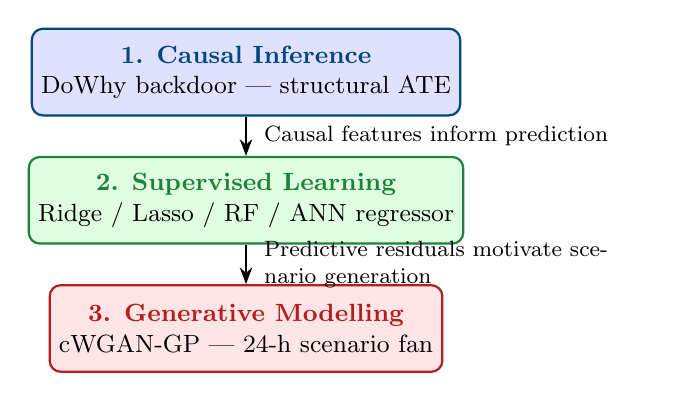
\begin{tikzpicture}[
  node distance=0.4cm,
  box/.style={rectangle, rounded corners=4pt, draw, thick,
              minimum width=3.8cm, minimum height=1.1cm,
              align=center, font=\small},
  arr/.style={-{Stealth[length=6pt]}, thick},
  label/.style={font=\footnotesize, text width=4.8cm}
]
  \node[box, fill=blue!12, draw=dblue] (ci)
    {\textbf{\textcolor{dblue}{1. Causal Inference}}\\
     DoWhy backdoor — structural ATE};

  \node[box, fill=green!12, draw=dgreen, below=0.5cm of ci] (sl)
    {\textbf{\textcolor{dgreen}{2. Supervised Learning}}\\
     Ridge / Lasso / RF / ANN regressor};

  \node[box, fill=red!10, draw=dred, below=0.5cm of sl] (gen)
    {\textbf{\textcolor{dred}{3. Generative Modelling}}\\
     cWGAN-GP — 24-h scenario fan};

  \draw[arr] (ci) -- (sl)
    node[midway, right=0.1cm, label]
    {\footnotesize Causal features inform prediction};
  \draw[arr] (sl) -- (gen)
    node[midway, right=0.1cm, label]
    {\footnotesize Predictive residuals motivate scenario generation};

\end{tikzpicture}

\vspace{0.4em}
\small
Each block answers a distinct question; together they form a
\textbf{connected evidence chain} from mechanism to policy action.
The causal block identifies \emph{what drives demand}; the supervised
block \emph{quantifies future levels}; the generative block
\emph{stress-tests grid capacity} under unseen heat extremes.

\end{column}
\end{columns}

\end{frame}

% ══════════════════════════════════════════════════════════════════════════════
%  SLIDE 3 — Results: Causal Inference
% ══════════════════════════════════════════════════════════════════════════════
\begin{frame}{3 \;|\; Results — Causal Inference}

\begin{columns}[T]
\begin{column}{0.54\textwidth}

\textbf{Step 1 — identify the structural mechanism}

DoWhy backdoor adjustment on 87,672 hourly observations yields:
\[
  \widehat{\text{ATE}} = \mathbf{268.23\text{ MW / THI unit}}
\]
Controlling for \texttt{hour, dow, month, cloud\_pct, wind\_ms, precip\_mm}.
Refutation p-value = 0.96 — estimate is robust.

\vspace{0.6em}
\textbf{Step 2 — reveal the non-linear acceleration}

Quadratic structural form ($R^2 = 0.59$):
\[
  \hat{y} = 23{,}500 - 689.80\,(\text{THI}) + 6.53\,(\text{THI}^2) + \mathbf{\Gamma X}
\]
Marginal Causal Effect:
\[
  \text{MCE}(\text{THI}) = -689.80 + 13.06\cdot\text{THI}
\]


\end{column}
\begin{column}{0.43\textwidth}

\textbf{MCE by operating scenario}

\vspace{0.3em}
\begin{tabular}{@{}lcc@{}}
\toprule
Scenario & THI & MCE (MW/unit) \\
\midrule
Mild summer day      & 65   & 159.4 \\
Mean summer baseline & 73.3 & \textbf{268.2} \\
Severe heatwave      & 82   & 381.5 \\
\bottomrule
\end{tabular}

\vspace{0.7em}
\textbf{Policy implication}

A heatwave swing of THI 78 $\to$ 83:
 $ \emph{MCE} $\int_{78}^{83}\text{MCE}\,d\text{THI} = 1{,}677$ MW $

\vspace{0.4em}
\textbf{Refutation tests}

\begin{tabular}{@{}lc@{}}
\toprule
Test & Outcome \\
\midrule
Random common cause & Stable ($p=0.96$) \\
Placebo treatment   & Effect $\approx 0$ \\
Data subset (80\%)  & Consistent \\
\bottomrule
\end{tabular}

\end{column}
\end{columns}

\end{frame}

% ══════════════════════════════════════════════════════════════════════════════
%  SLIDE 4 — Results: Supervised Learning & Generative Modelling
% ══════════════════════════════════════════════════════════════════════════════
\begin{frame}{4 \;|\; Results — Prediction \& Scenario Generation}

\begin{columns}[T]
\begin{column}{0.50\textwidth}

\textbf{From mechanism to prediction}

The causal block told us \emph{why} demand rises with THI.
The supervised block asks: \emph{can we forecast how much?}
THI, hour, month, and weather confounders — identified causally — become
the feature set.

\vspace{0.5em}
\begin{tabular}{@{}lcc@{}}
\toprule
Model & RMSE (MW) & $R^2$ \\
\midrule
Ridge / Lasso & 2,183 & 0.531 \\
ANN           & 1,637 & 0.736 \\
\textbf{Random Forest} & \textbf{1,562} & \textbf{0.760} \\
\bottomrule
\multicolumn{3}{@{}l@{}}{\footnotesize Hold-out: 2024–2025 (17,544 obs)} \\
\end{tabular}

\vspace{0.5em}
\small
Random Forest captures non-linear interactions (notably THI $\times$ hour)
that linear estimators miss — consistent with the accelerating MCE we
identified causally. Cross-validation $R^2 = 0.720 \pm 0.041$ across
5 temporal folds confirms robustness beyond the train window.

\end{column}
\begin{column}{0.47\textwidth}

\textbf{From prediction to scenario generation}

Even the best model gives a \emph{point forecast}. For capacity planning,
utilities need \emph{probabilistic scenario fans}. The cWGAN-GP generates
10+ 24-hour demand profiles conditioned on:
\vspace{-.2 em}
\begin{itemize}
  \item Previous day's actual demand (24 values)
  \vspace{-.2 em}
  \item Previous \& current day's weather (24 h $\times$ 5 vars each)
\end{itemize}
\vspace{-.2 em}
\begin{tabular}{@{}lc@{}}
\toprule
Metric & Result \\
\midrule
Wasserstein Distance    & $870.8 \pm 583.4$ MW \\
Jensen-Shannon Div.     & $0.0021 \pm 0.0032$ \\
JS $\leq$ 0.05 check & \textcolor{dgreen}{\textbf{\checkmark\ Passed}} \\
Hold-out days evaluated & 306 (2024–2025) \\
\bottomrule
\end{tabular}

\small
\vspace{.2 em}
JS divergence $< 0.05$ confirms that generated profiles are
\textbf{statistically indistinguishable in shape} from real demand curves
— suitable for heatwave stress-testing and reserve margin planning.

\end{column}
\end{columns}

\end{frame}

% ══════════════════════════════════════════════════════════════════════════════
%  SLIDE 5 — Limitations & Synthesis
% ══════════════════════════════════════════════════════════════════════════════
\begin{frame}{5 \;|\; Limitations \& Synthesis}

\begin{columns}[T]
\begin{column}{0.52\textwidth}

\textbf{The connected evidence chain}

\begin{enumerate}
  \item \textbf{Causal Inference} established the structural mechanism:
        a monotonically accelerating MCE (159 $\to$ 381 MW/THI-unit)
        with a 336 MW underestimation penalty from linear models.
  \item \textbf{Supervised Learning} operationalised the causal insight:
        THI-based features lift $R^2$ from 0.53 (linear) to 0.76 (RF),
        confirming that the causal signal is also the dominant predictive signal.
  \item \textbf{Generative Modelling} extended point forecasts to probabilistic
        scenario fans: JS divergence $= 0.002$ proves distributional realism
        across 306 unseen hold-out days.
\end{enumerate}


\end{column}
\begin{column}{0.45\textwidth}

\textbf{Limitations}

\begin{itemize}
  \item \textbf{Unobserved confounders:} kharif irrigation pump schedules,
        industrial load contracts, and public holidays are excluded and
        may inflate the causal THI estimate

  \item \textbf{GAN tail coverage:} WGAN-GP may under-represent extreme
        demand-spike events despite gradient penalty regularisation
 
\end{itemize}
\vspace{-.6 em}
\begin{alertblock}{Conclusion}
\small
A one-unit rise in THI causes a structural \textbf{268 MW average demand
increase}; under heatwave conditions this accelerates to \textbf{381 MW/unit}.
Causal-feature-informed Random Forest forecasts reach $R^2 = 0.76$, and
cWGAN-GP generates distributional-realistic capacity-planning scenarios.
\end{alertblock}
\end{column}
\end{columns}

\end{frame}

% ══════════════════════════════════════════════════════════════════════════════
%  REFERENCES
% ══════════════════════════════════════════════════════════════════════════════
\begin{frame}{References}

\small
\begin{thebibliography}{9}

\bibitem{dowhy}
Sharma, A., \& Kiciman, E. (2020).
DoWhy: An end-to-end library for causal inference.
\emph{arXiv:2011.04216}.

\bibitem{wgangp}
Gulrajani, I., Ahmed, F., Arjovsky, M., Dumoulin, V., \& Courville, A. (2017).
Improved training of Wasserstein GANs.
\emph{Advances in Neural Information Processing Systems, 30}.

\bibitem{sklearn}
Pedregosa, F., et al.\ (2011).
Scikit-learn: Machine learning in Python.
\emph{Journal of Machine Learning Research, 12}, 2825--2830.

\bibitem{iced}
NITI Aayog. (2025).
\emph{India Climate Energy Dashboard (ICED) — Load Curve Portal}.
\texttt{https://iced.niti.gov.in}

\bibitem{nasapower}
Stackhouse, P.\ W., et al.\ (2018).
NASA POWER: Agroclimatology parameters for sustainable development.
\emph{Bulletin of the American Meteorological Society}.

\bibitem{pearl}
Pearl, J. (2009).
\emph{Causality: Models, Reasoning, and Inference} (2nd ed.).
Cambridge University Press.

\end{thebibliography}

\end{frame}

% ══════════════════════════════════════════════════════════════════════════════
%  BACKUP SLIDES — tables and figures only
% ══════════════════════════════════════════════════════════════════════════════

\begin{frame}{Backup — Causal DAG}
\centering
\begin{tikzpicture}[
  node distance=1.2cm and 1.8cm,
  every node/.style={font=\small},
  obs/.style={circle, draw=dblue, thick, minimum size=0.85cm, fill=blue!8},
  treat/.style={circle, draw=dred, thick, minimum size=0.85cm, fill=red!10},
  out/.style={circle, draw=dgreen, thick, minimum size=0.85cm, fill=green!10},
  arr/.style={-{Stealth[length=6pt]}, thick}
]
  \node[obs] (month) {month};
  \node[obs, below left=1cm and 0.9cm of month] (tc) {temp\_c};
  \node[obs, below right=1cm and 0.9cm of month] (rh) {rh\_pct};
  \node[treat, below=1cm of month] (thi) {\textbf{THI}};
  \node[obs, right=2.0cm of thi] (hour) {hour/dow};
  \node[obs, left=2.0cm of thi] (cloud) {cloud\_pct};
  \node[obs, below left=0.8cm and 1.6cm of thi] (wind) {wind\_ms};
  \node[obs, below right=0.8cm and 1.6cm of thi] (prec) {precip};
  \node[out, below=1.8cm of thi] (demand) {\textbf{demand\_mw}};

  \draw[arr] (month) -- (tc);
  \draw[arr] (month) -- (rh);
  \draw[arr] (tc) -- (thi);
  \draw[arr] (rh) -- (thi);
  \draw[arr] (thi) -- (demand);
  \draw[arr] (hour) -- (demand);
  \draw[arr] (cloud) -- (tc);
  \draw[arr] (cloud) -- (demand);
  \draw[arr] (wind) -- (demand);
  \draw[arr] (prec) -- (demand);
  \draw[arr, dashed, gray] (month) to[bend left=35] (demand);
  \draw[arr, dashed, gray] (hour) to[bend left=25] (tc);
\end{tikzpicture}

\vspace{0.4em}
\small
\textbf{Identification:} backdoor criterion satisfied by adjusting for
\{\texttt{rh\_pct, temp\_c}\} (minimal adjustment set per DoWhy).
Unconfoundedness assumption: no unmeasured common cause of THI and demand.
\end{frame}

\begin{frame}{Backup — Full Supervised Learning Results}

\centering
\textbf{5-Fold Temporal Cross-Validation}

\vspace{0.4em}
\begin{tabular}{@{}lcccc@{}}
\toprule
Model & RMSE (MW) & MAE (MW) & $R^2$ \\
\midrule
Ridge        & $2{,}176 \pm 105$ & $1{,}748 \pm 82$  & $0.513 \pm 0.033$ \\
Lasso        & $2{,}176 \pm 105$ & $1{,}748 \pm 82$  & $0.513 \pm 0.033$ \\
Random Forest & $1{,}647 \pm 154$ & $1{,}164 \pm 128$ & $0.720 \pm 0.041$ \\
ANN          & $1{,}685 \pm 144$ & $1{,}251 \pm 127$ & $0.708 \pm 0.039$ \\
\bottomrule
\end{tabular}

\vspace{0.9em}
\textbf{Final Hold-Out Test (2024–2025 | 17,544 observations)}

\vspace{0.4em}
\begin{tabular}{@{}lccc@{}}
\toprule
Model & RMSE (MW) & MAE (MW) & $R^2$ \\
\midrule
Ridge                    & 2,183.0 & 1,725.1 & 0.5312 \\
Lasso                    & 2,183.0 & 1,725.1 & 0.5312 \\
ANN                      & 1,637.1 & 1,165.9 & 0.7364 \\
\textbf{Random Forest}   & \textbf{1,562.2} & \textbf{1,119.8} & \textbf{0.7599} \\
\bottomrule
\end{tabular}

\vspace{0.5em}
\small Best RF hyperparameters: \texttt{n\_estimators=300, max\_depth=10}\\
Train period: 2016–2023 (70,128 obs) \quad Test period: 2024–2025 (17,544 obs)

\end{frame}

\begin{frame}{Backup — cWGAN-GP Architecture \& Training}

\centering
\textbf{Network Architecture}

\vspace{0.4em}
\begin{tabular}{@{}llll@{}}
\toprule
Component & Input dim & Hidden layers & Output \\
\midrule
\textbf{Generator} & 32 (noise) + 264 (cond) = 296 & 512 $\to$ 1024 $\to$ 512\ (ReLU + BN) & 24 (Tanh) \\
\textbf{Critic}    & 24 (demand) + 264 (cond) = 288 & 512 $\to$ 256 $\to$ 128\ (LeakyReLU 0.2) & 1 (unbounded) \\
\bottomrule
\end{tabular}

\vspace{0.9em}
\textbf{Training \& Evaluation Summary}

\vspace{0.4em}
\begin{tabular}{@{}ll@{}}
\toprule
Hyperparameter / Metric & Value \\
\midrule
Epochs & 300 \quad Batch size: 64 \\
Optimiser & Adam ($\eta=10^{-4}$, $\beta_1=0.5$, $\beta_2=0.9$) \\
Critic steps / generator step & 5 \quad Gradient penalty $\lambda=10$ \\
Condition dim & 264 (24 lag-demand + 120 lag-weather + 120 curr-weather) \\
Data augmentation & Gaussian jitter 2–3\% $\sigma$, $\times 3$ copies \\
Train days & 1,223 (2016-04-02 $\to$ 2023-08-31), 3,669 after augmentation \\
Hold-out days & 306 (2024-04-01 $\to$ 2025-08-31), 10 scenarios/day \\
\midrule
Wasserstein Distance (MW) & $870.8 \pm 583.4$ \\
Jensen-Shannon Divergence & $0.0021 \pm 0.0032$ \\

\bottomrule
\end{tabular}

\end{frame}

\begin{frame}{Backup — Full Variable Specification}

\centering
\small
\begin{tabular}{@{}llll@{}}
\toprule
Variable & Type & Role & Description \\
\midrule
\texttt{datetime}   & Temporal index   & Identifier         & YYYY-MM-DD HH:00:00 \\
\texttt{demand\_mw} & Continuous float & \textbf{Outcome}   & Punjab grid consumption (MW) \\
\texttt{thi}        & Continuous float & \textbf{Treatment} & Temperature-Humidity Index \\
\texttt{temp\_c}    & Continuous float & Upstream cause     & 23-station avg.\ temperature (°C) \\
\texttt{rh\_pct}    & Continuous float & Upstream cause     & 23-station avg.\ humidity (\%) \\
\texttt{precip\_mm} & Continuous float & Covariate          & Hourly precipitation (mm) \\
\texttt{cloud\_pct} & Continuous float & Confounder         & Cloud cover (\%) \\
\texttt{wind\_ms}   & Continuous float & Covariate          & Wind speed (m/s) \\
\texttt{hour}       & Integer          & Fixed effect       & Hour of day (0–23) \\
\texttt{dow}        & Integer          & Fixed effect       & Day of week (0–6) \\
\texttt{month}      & Integer          & Fixed effect       & Month (1–12) \\
\texttt{year}       & Integer          & Fixed effect       & Year (2016–2025) \\
\bottomrule
\end{tabular}

\vspace{0.7em}
\textbf{Dataset dimensions:} 87,672 hourly obs $\times$ 12 variables \quad
\textbf{Panel:} 2016–2025 \quad
\textbf{Scope:} 23 Punjab districts \quad
\textbf{THI range:} 37.1–89.9 \quad
\textbf{Demand range:} 1,793–18,441 MW

\end{frame}

\end{document}
